%!TEX root = ../dokumentation.tex

\chapter{Trainieren eines Klassifikationsmodells} \label{ch:crispDm_1}

In dem folgenden Abschnitt wird \ac{CRISP-DM} genutzt, um \ac{ML} Modelle zu trainieren, welche Texte einer der sechs politischen Parteien aus dem Deutschen Bundestag zuordnet. 

% TODO: Add missing sections

\ac{CRISP-DM} ist ein weitverbreitetes iteratives Modell, welches zur Strukturierung von Data-Mining Projekten genutzt wird \autocite{martinez-plumed_casp-dm_2017, chapman_crisp-dm_2000}. Das Modell besteht aus sechs Schritten: Business Understanding, Data Understanding, Data Preparation, Modeling, Evaluation und Deployment. 

\begin{figure}[H]
    \centering
    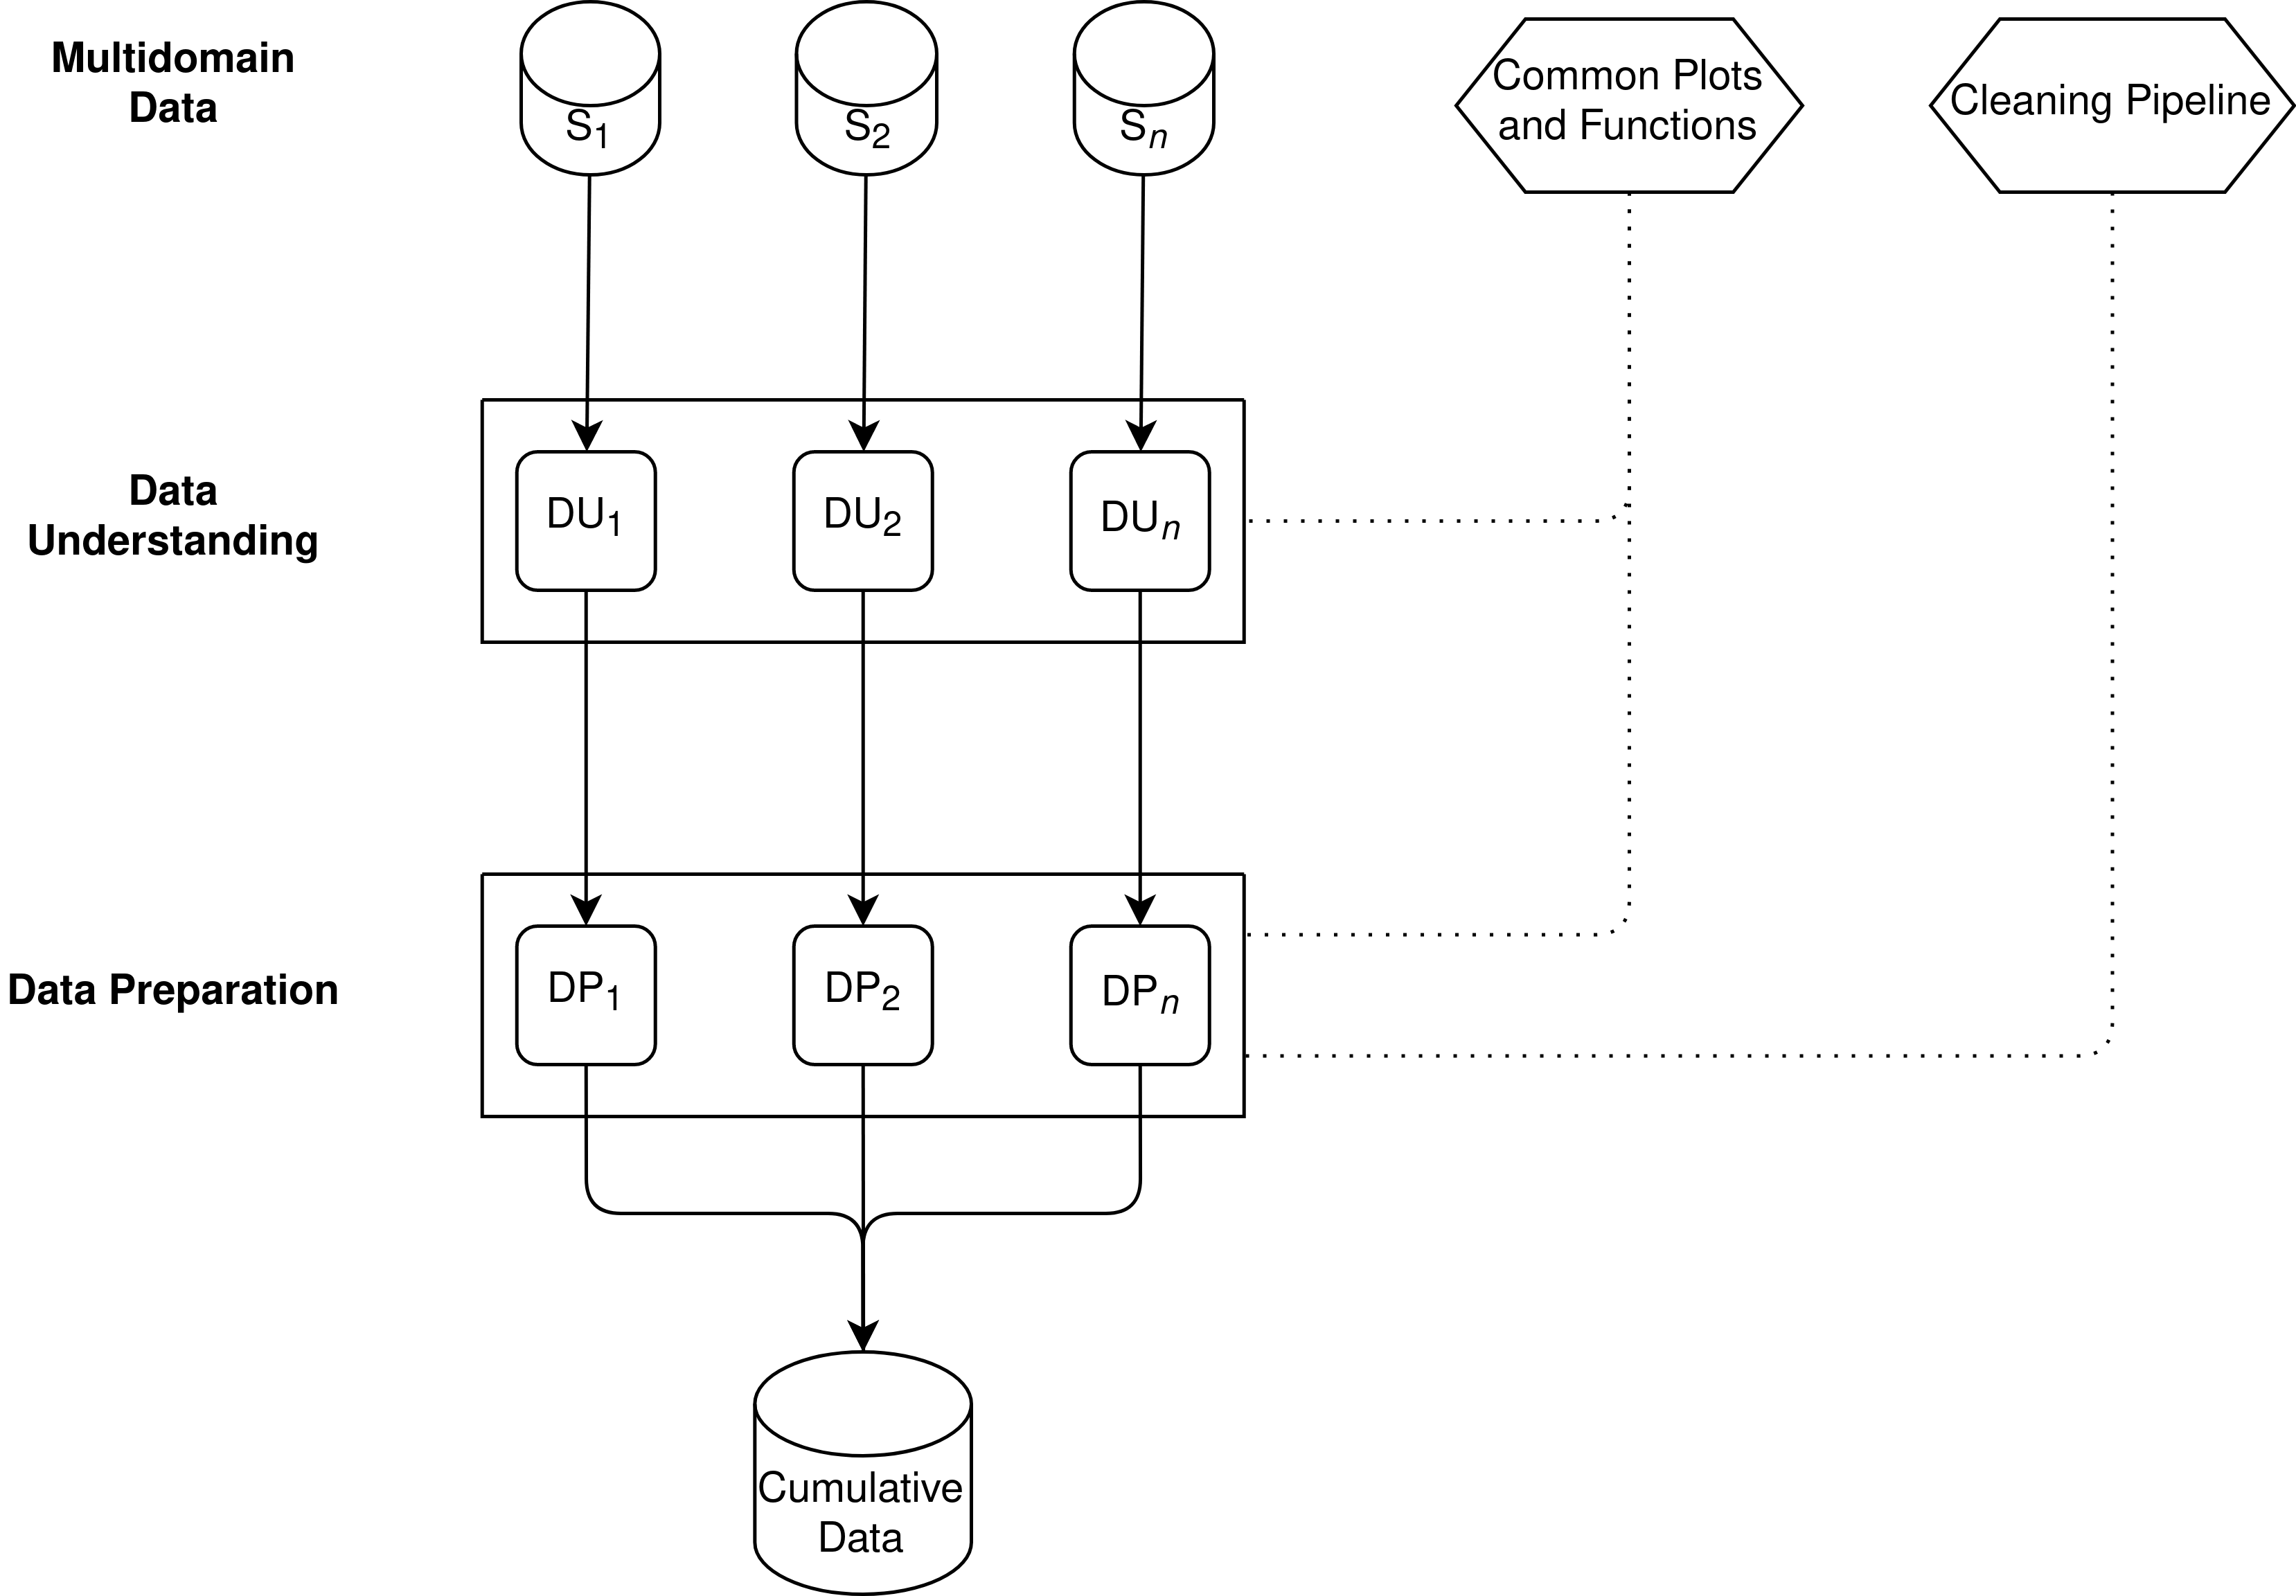
\includegraphics[width=0.8\textwidth]{data/images/data_flow_v2_1.png}
    \caption[Datenverarbeitungs-Pipeline]{Datenverarbeitungs-Pipeline (Data Understanding, Data Preparation und Zusammenführung der Daten)} \label{fig:dataFlow_1}
\end{figure}

% TODO: Add source for multidomain data

Multidomain Daten ermöglichen es, generalisierter \ac{ML} Modelle zu trainieren. Da die Rohdaten stark voneinander abweichen, ist es notwendig, dass unterschiedliche Datenquellen im Prozess des Data Understandings und Data Preparation individuell verarbeitet werden. Nachdem jeder Datensatz einzeln analysiert und bereinigt wurde, werden die Daten für das Modeling zusammengeführt.

% TODO: Update image for modeling

\begin{figure}[H]
    \centering
    \missingfigure
    \caption[Training von Modellen]{Training von Modellen (Modeling)} \label{fig:dataFlow_2}
\end{figure}

Lorem Ipsum

\section{Sichtung der ausgewählten Datenquellen} \label{sec:dataUnderstanding}

Wie zuvor beschrieben, werden in dieser Arbeit verschiedene Datensätze genutzt, um die \ac{ML} Modelle zu trainieren. Damit soll vermieden werden, dass ein Modell lediglich die Eigenschaften eines spezifischen Datensatzes trainiert. 

Für das \nameref{sec:modeling} werden Datensätze benötigt, welche neben den Features (z. B. Text, Alter, Geschlecht) auch einer Partei zugeordnet sind. Da in dieser Form noch keine Datensätze vorhanden waren, wurden explizit Daten gewählt, welche von Politikern einer Partei veröffentlicht wurden. Somit kann die Parteizugehörigkeit als Zielvariable für das Training genutzt werden.

% TODO: Update values

\begin{table}[H]
    \centering
    {\footnotesize
    \begin{tblr}{width=\textwidth, hlines, vlines}
        \textbf{Datensatz} & \textbf{AfD} & \textbf{Die Grünen} & \textbf{SPD} & \textbf{Union} & \textbf{Die Linke} & \textbf{FDP} & \textbf{Gesamt\-anzahl} \\ 

        Tweets\footnote{Tweets von den aufgeführten Parteien, exklusive parteilose Politiker} & \num{126132} & \num{167060} & \num{167647} & \num{157035} & \num{141738} & \num{112067} & \num{871679} \\
        Reden\footnote{Reden von den aufgeführten Parteien in dem Zeitraum der 19. Legislaturperiode.} & \num{4437} & \num{3857} & \num{5249} & \num{8007} & \num{3403} & \num{3888} & \num{28841} \\
        Wahlpro\-gramme & \num{2619} & \num{6399} & \num{4552} & \num{4564} & \num{5204} & \num{4376} & \num{27714} \\

        \textbf{Summe} & \textbf{\num{133188}} & \textbf{\num{176861}} & \textbf{\num{177448}} & \textbf{\num{170246}} & \textbf{\num{150345}} & \textbf{\num{120331}} & \textbf{\num{928234}} \\
    \end{tblr}
    }
    \caption{Anzahl an Einträgen pro Datensatz und pro Partei vor Bereinigen und Filtern} \label{tab:countPerDataset}
\end{table}

% TODO: Update number

Bei den Datensätzen handelt es sich um Tweets, Wahlprogramme (Landtags-, Europa- und Bundestagswahlen) und Reden aus dem Deutschen Bundestag. Wie aus \autoref{tab:countPerDataset} hervorgeht, umfassen die drei Datensätze initial \num{928234} Einträge. 

\subsection*{Tweets}

% TODO: Add source

Twitter ist eine amerikanische Kurznachrichten-Plattform, welche den Nutzern ermöglicht, Tweets\footnote{Plattformspezifische Bezeichnung für Kurznachrichten} von einer Länge von bis zu 280 Zeichen zu veröffentlichen. Zusätzlich zum Veröffentlichen von eigenen Tweets, besitzen Nutzer die Möglichkeit Tweets von anderen zu kommentieren, oder zu retweeten\footnote{Einen Tweet eines anderen Nutzers auf seinem eigenen Profil erneut veröffentlichen}.

Der Tweet-Datensatz\footnote{Aufgrund der Twitter Developer Bedingungen ist der Datensatz nicht öffentlich zugänglich. \citeauthor{saltzer_finding_2022} hat auf Anfrage den Datensatz für diese Arbeit zur Verfügung gestellt.} von \textcite{saltzer_finding_2022} umfasst \num{876118} Tweets von \num{511} Politikern des Deutschen Bundestages zwischen Januar \num{2017} bis Dezember \num{2019}. 

Der Datensatz beinhaltet neben den Tweet-Texten (\texttt{text}) auch noch den Twitternamen (\texttt{screen\_name}), das Erstellungsdatum (\texttt{created\_at}), ob es sich um einen Retweet handelt (\texttt{is\_retweet}), welcher Partei der Politiker angehört (\texttt{party}), das Geburtsdatum (\texttt{birthyear}) und das Geschlecht des Politikers (\texttt{gender}). Initial beinhaltet der Datensatz außerdem noch, ob der Politiker einer Untergruppierung einer Partei angehört und wie dieser bei Abstimmungen im Deutschen Bundestag abgestimmt hat. Diese letzten beiden Informationen werden jedoch im folgenden nicht weiter berücksichtigt.

Die Tweets der Parlamentarier lassen sich folgenden sechs Parteien\footnote{Initial beinhaltete der Datensatz zusätzlich Parteilose, welche jedoch direkt gefiltert wurden.} zuordnen: Die Grünen, \ac{SPD}, Die Linke, \ac{AfD}, \ac{FDP} und Union. Unter den \ac{MdB} befinden sich \num{161} Frauen und \num{350} Männer.

% TODO: Update image with correct image (pre-processing)

\begin{figure}[H]
    \centering
    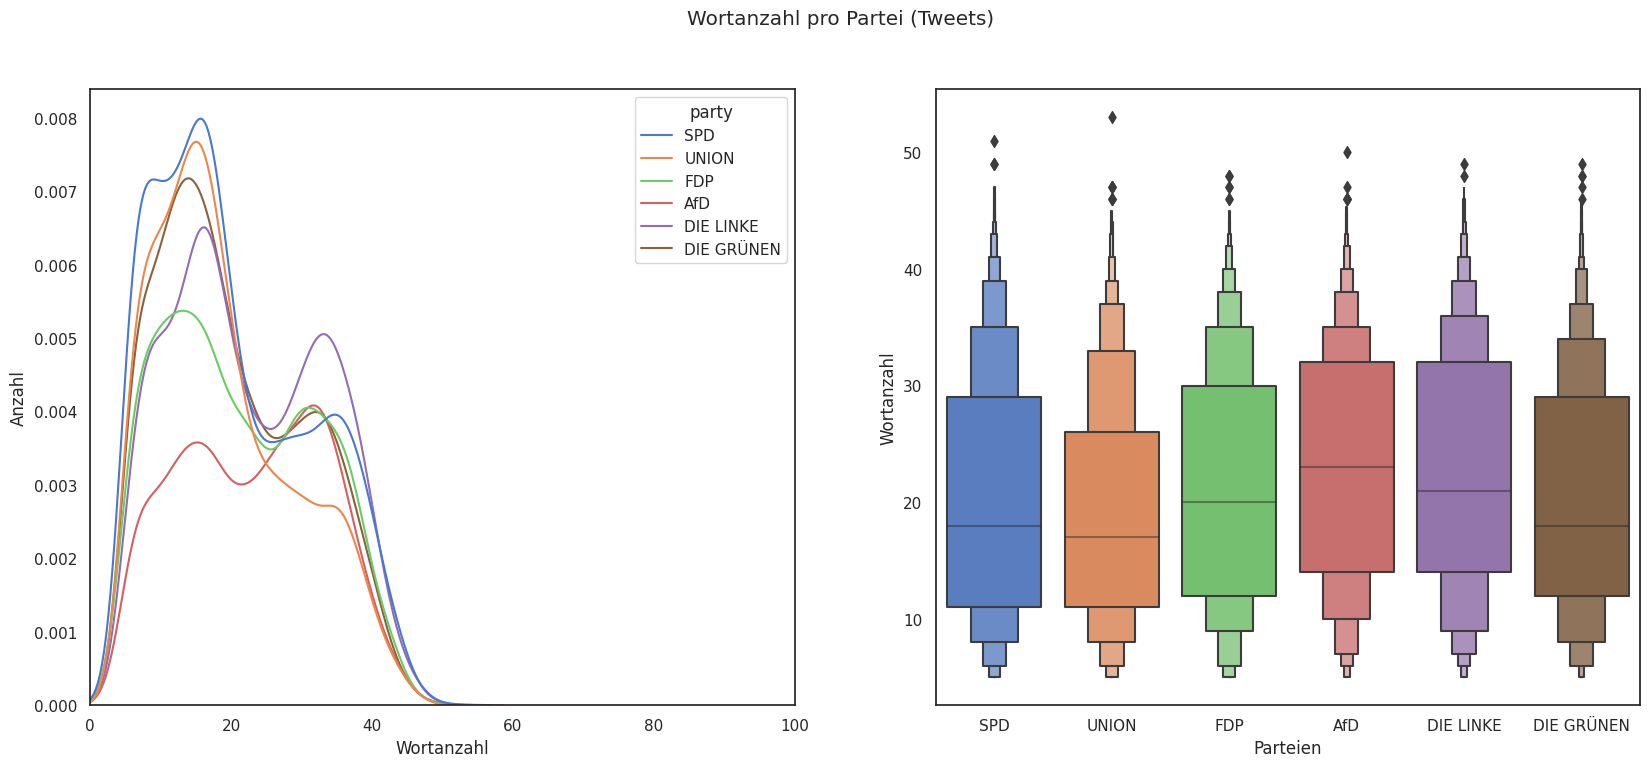
\includegraphics[width=0.9\textwidth]{data/images/tweets_word_count.png}
    \caption{Anzahl an Wörtern für Tweets vor Bereinigung} \label{fig:wordCoundTweets}
\end{figure}

% TODO: Add reference

\autoref{fig:wordCoundTweets} zeigt eine Dichtefunktion der Wortanzahl der Tweets gruppiert nach den einzelnen Parteien. Diese weisen jeweils zwei Extrema auf. Das Erste befindet sich im Bereich zwischen \num{15} bis \num{25} Wörtern und das Zweite im Bereich zwischen \num{30} bis \num{40} Wörtern. Im Durchschnitt veröffentlichen Politiker der Union vergleichsweise kurze Nachrichten, wohingegen die der \ac{AfD}, der \ac{FDP} und die der Linken vermehrt längere Nachrichten veröffentlichen.

\subsection*{Reden} \label{subsec:dataUnderstandingReden}

Als weitere Datenquelle sollen politische Reden, die von den Abgeordneten der verschiedenen Fraktionen im Bundestags gehalten worden sind, genutzt werden. Dabei kann auf den Datensatz \enquote{Open Discourse} von \textcite{richter_open_2021} zurückgegriffen werden, der alle Plenarprotokolle des Deutschen Bundestages von \num{1949} bis \num{2020} in Textform zur Verfügung stellt.

Neben den Reden, die im Folgenden als Trainingsdaten genutzt werden sollen, enthält der Datensatz auch alle Zwischenrufe und -fragen, die von Parlamentariern während der Debatten geäußert wurden. Aufgrund von mangelnder Qualität und Länge dieser werden sie für den weiteren Verlauf der Arbeit als Datenquelle verworfen.

Zusätzlich zum Text (\texttt{speechContent}) liegen für jede Rede unter anderem zusätzlich die Nummer der Sitzung des Bundestages (\texttt{session}), das Datum (\texttt{date}), Vor- und Nachname (\texttt{firstName} bzw. \texttt{lastName}), die Fraktion (\texttt{factionId}) sowie die Position des Redners (\texttt{positionLong}) vor.

Über alle Wahlperioden hinweg enthält der Datensatz insgesamt \num{907644} Reden von \num{4105} Politikern. Da sich das zu trainierende Klassifikationsmodell im Rahmen dieser Arbeit nur auf die 19. Wahlperiode bezieht, werden nur Reden berücksichtigt, die auch in dem genannten Zeitraum gehalten wurden, wodurch noch \num{60958} Reden übrig bleiben. Die übrigen Reden umfassen jedoch auch Beiträge des Präsidiums des Deutschen Bundestages sowie fraktionsloser Abgeordneter, die beide nicht betrachtet werden können, da sie keiner der definierten Parteien zuzuordnen sind. Somit reduziert sich die Zahl an Reden schlussendlich auf \num{28841}.

% TODO: Verteilung der Reden nach Partei

\begin{figure}[H]
    \centering
    \includegraphics[width=0.9\textwidth]{data/images/speeches_word_count.png}
    \caption{Anzahl an Wörtern für Reden vor Bereinigung} \label{fig:wordCoundSpeeches}
\end{figure}

\autoref{fig:wordCoundSpeeches} zeigt die Verteilung der Anzahl an Wörtern, die die Reden im Datensatz umfassen, aufgeschlüsselt nach Partei. Es ergibt sich dabei ein Hochpunkt in der Dichtefunktion bei knapp unter 100 Wörtern, gefolgt von einem Tiefpunkt zwischen \num{200} und \num{300} Wörtern und schließlich einem weiteren Hochpunkt, je nach Partei zwischen 400 und 700 Wörtern.

Dies zeigt, dass die Reden im Durchschnitt etwa um den Faktor zehn länger sind als Tweets, was darauf zurückzuführen ist, dass die Reden im Bundestag oft mehrere Minuten andauern, während Tweets als Kurznachrichten gedacht sind.

Bei genauerer Betrachtung der Häufung von kurzen Reden rund um das erste Maximum fällt auf, dass dort viele Redebeiträge enthalten sind, die nur beispielsweise Zwischenfragen darstellen und keine vollständigen, inhaltlich relevanten Reden sind.

% TODO: Beispiele für kurze Reden / Zwischenfragen im Anhang

\subsection*{Wahlprogramme}

Zuletzt sollen auch Texte aus Wahlprogrammen der zu untersuchenden Parteien herangezogen werden. Dabei stehen im Untersuchungszeitraum die Bundestagswahlen \num{2017} und \num{2021}, die Europawahl 2019 sowie zahlreiche Landtagswahlen mit den entsprechend veröffentlichten Wahlprogrammen der Parteien zur Verfügung. Eine genaue Auflistung der verwendeten Wahlen inklusive Anmerkungen zu Wahlprogrammen, die nicht verarbeitet werden konnten, kann dem \autoref{subsec:übersichtWP} im Anhang entnommen werden.

So ergibt sich eine Anzahl von insgesamt \num{83} Wahlprogrammen unterschiedlicher Parteien. Damit aus den Wahlprogrammen kohärente, kürzere Texte extrahiert werden können, wird jedes Wahlprogramm nach Absätzen unterteilt, sodass sich eine Gesamtanzahl von \num{28783} Paragraphen als Trainingsdaten vor der Bereinigung ergibt.

% TODO: kurz beschreiben, wie das Parsing abläuft

Neben dem Text des jeweiligen Paragraphen liegen als weitere Informationen, die während des Auslesens der Wahlprogramme gesammelt wurden, die Partei, aus deren Wahlprogramm der Text entnommen wurde (\texttt{party}), die Art der Wahl (\texttt{election\_type})\footnote{Bundestags-, Europa- oder Landtagswahl} und ein Kürzel für die Wahl (\texttt{election})\footnote{Bestehend aus Art der Wahl, gegebenenfalls Bundesland und Jahr} vor.

\begin{figure}[H]
    \centering
    \includegraphics[width=0.9\textwidth]{data/images/party_programs_word_count.png}
    \caption{Anzahl an Wörtern für Wahlprogramm-Paragraphen vor Bereinigung} \label{fig:wordCoundPartyPrograms}
\end{figure}

\autoref{fig:wordCoundPartyPrograms} zeigt die Verteilung der Anzahl an Wörtern der gewonnenen Wahlprogramm-Paragraphen pro Partei. Anders als bei den Reden zeigt sich hier eine rechtsschiefe Dichtefunktion mit nur einem Maximum bei -- je nach Partei -- etwa \num{30} bis \num{70} Wörtern pro Paragraph. Damit sind die Absätze aus Wahlprogrammen durchschnittlich länger als die Tweets, jedoch deutlich kürzer als die Transkripte der Bundestagsreden. 


\section{Datenaufbereinigung} \label{sec:dataPreparation}

% TODO: Check if there are limitations in using Doc2Vec, Sentence2Vec und Word2Vec

\subsection{Datenbereinigungs-Pipeline} \label{subsec:cleaningPipeline}

Stopwörter, Links, Symbole und weitere Unregelmäßigkeiten (Rauschen, zu Englisch \textit{Noise}) beeinflussen die Performance von \ac{ML} Modellen stark \autocite[4]{kowsari_text_2019}. Daher ist es notwendig Texte mittels regelbasierten Verfahren, als auch mit \ac{ML} Verfahren zu bereinigen. 

% TODO: Add more details for "Regelbasiertes Bereinigen" and add tokenizing to stemming
% TODO: Rename Stemming to Lemmatizing

\begin{figure}[H]
    \centering
    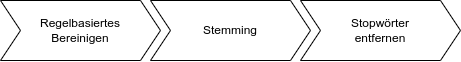
\includegraphics[width=0.7\linewidth]{data/images/cleaning_pipeline_v1.png}
    \caption{Datenbereinigungsprozess} \label{fig:cleaningPipeline}
\end{figure}

Wie \autoref{fig:cleaningPipeline} zeigt, besteht der Prozess zur Datenbereinigung aus drei Abschnitten. Zuerst die regelbasierte Bereinigung, welche mittels regulären Ausdrücken und Patterns eine erste Umformung vornimmt. Im nächsten Schritt werden die Wörter auf ihren Wortstamm zurückgeführt. Im letzten Schritt werden Stopwörter entfernt. All diese Schritte verfolgen das Ziel, die Menge an Rauschen zu verringern. 

\subsubsection{Regelbasierte Verfahren}

Unterschiedliche Schreibweisen, Symbole und Emojis, \acp{URL}, und Gendern stellen ein elementares Problem für herkömmliche \ac{NLP} Methoden und Modelle dar. Im ersten Schritt werden daher regelbasierte Verfahren genutzt, um häufig auftretende Zeichen, Symbole/Emojis, aber auch andere Unregelmäßigkeiten ersetzt oder entfernt.

Speziell bei Tweets werden häufig Symbole wie \euro und \& als Kurzform verwendet. Da diese jedoch nicht in dieser Form interpretiert werden können, werden die Symbole als auch die Zahlen mit ihrem ausgeschriebenen Klartext ersetzt. So wird aus \euro \(\rightarrow\) \textit{euro}, oder aus \(\num{2000} \rightarrow\) \textit{zweitausend}.

In den Texten treten vermehrt Unicode, \ac{HTML} Symbole, als auch Emojis auf. In Tweets als auch in Wahlprogrammen werden ebenfalls \acp{URL} verwendet. Tweets nutzen außerdem Referenzen zu Twitternutzern (Mentions wie \textit{@MaxMustermann}). Da es sich bei all diesen Symbolgruppen um nicht vollständige oder nicht interpretierbare Zeichenketten handelt, müssen diese entfernt werden.

Bei allen Textformen verwenden Politiker und Parteien unterschiedliche Arten von inklusiver Sprache als Alternative zum generischen Maskulinum. Beispiele hierfür sind \textit{Politiker*innen} oder auch \textit{Politiker:innen}. Da die Textrepräsentationsformen und Sprachmodelle dies jedoch nur rudimentär oder gar nicht abbilden können, werden alle herkömmlichen Endungen für gendergerechte Sprache entfernt, sodass alle Wörter im Text auf den korrekten Wortstamm reduziert werden können.

Nachdem die Texte grob bereinigt wurden, werden letztlich noch Satzzeichen, Sonderzeichen und einzelne Buchstaben entfernt. Abschließend werden doppelte Leerzeichen entfernt und alle Buchstaben zu Kleinbuchstaben umgewandelt.

Bei den Redetexten ist zusätzlich zu beachten, dass im Datensatz Zwischenrufe von anderen Politikern im Redetext durch Referenzen -- gekennzeichnet durch eine Zahl innerhalb geschweifter und normaler Klammern -- vorkommen. Da der Text nur den Inhalt der Rede selbst beinhalten soll, werden die Referenzen zu den Zwischenrufen mithilfe eines regulären Ausdrucks entfernt.

% TODO: Zur Bereinigung der Wahlprogramm-Texte \dots

% TODO: Update tweet example

\begin{code}[H]
    \begin{minipage}{0.45\textwidth}
        \small
        \textcolor{orange}{Ehemalige} \textcolor{red}{@AfD-Vorsitzende} \textcolor{orange}{\#Petry} muss wegen \textcolor{orange}{Meineid} vor \textcolor{orange}{Gericht}\textcolor{red}{.} \textcolor{orange}{Kein Einzelfall}\textcolor{red}{:} gegen circa \textcolor{orange}{\SI{10}{\percent}} aller \textcolor{orange}{AfD-Abgeordneten} bundesweit laufen oder liefen \textcolor{orange}{Strafverfahren}\textcolor{red}{.} \textcolor{orange}{Kriminelle Asylbewerber}\textcolor{red}{?} \textcolor{orange}{Fehlanzeige}\textcolor{red}{.} \textcolor{orange}{Kriminelle AfD-Hetzer} trifft den \textcolor{orange}{Nagel} eher auf den \textcolor{orange}{Kopf} \textcolor{red}{<U+0001F602>} \textcolor{orange}{\#AfD}
    \end{minipage}\hfill
    \begin{minipage}{0.45\textwidth}
        \small
        ehemalige petry muss wegen meineid vor gericht kein einzelfall gegen circa zehn prozent aller afd abgeordneten bundesweit laufen oder liefen strafverfahren kriminelle asylbewerber fehlanzeige kriminelle afd hetzer trifft den nagel eher auf den kopf afd
    \end{minipage}\hfill
    \caption[Beispiel -- Regelbasierte Bereinigung]{Beispiel für regelbasierte Bereinigung eines Tweets von \textit{victorperli} (links befindet sich der Ausgangstext und rechts der Text nach der regelbasierten Bereinigung)} \label{list:rulebasedCleaning}
\end{code}

\autoref{list:rulebasedCleaning} zeigt die Anwendung der regelbasierten Bereinigung auf einen Beispiel-Tweet. Es lässt sich erkennen, dass die Referenz \textit{@AfD-Vorsitzende} im bereinigten Text nicht mehr vorkommt. Zudem wurde das Hashtag-Symbol vor \textit{Petry} und \textit{AfD} entfernt. Auch die Angabe \textit{10\%} wird durch die Bereinigung ausgeschrieben zu \textit{zehn prozent}. Schließlich enthält der bereinigte Text auf der rechten Seite keine Satzzeichen mehr, das Emoji am Ende fehlt und alle Wörter sind kleingeschrieben, sodass nur noch korrekte Wörter vorkommen.

\subsubsection{Stemming}

Lorem Ipsum

% TODO: Update tweet example

\begin{code}[H]
    \begin{minipage}{0.45\textwidth}
        \small
        \textcolor{orange}{ehemalige} petry muss wegen meineid vor gericht kein einzelfall gegen circa zehn prozent aller afd \textcolor{orange}{abgeordneten} bundesweit laufen oder liefen \textcolor{orange}{strafverfahren} \textcolor{orange}{kriminelle} asylbewerber \textcolor{orange}{fehlanzeige} \textcolor{orange}{kriminelle} afd hetzer \textcolor{orange}{trifft} \textcolor{orange}{den} nagel eher auf den kopf afd
    \end{minipage}\hfill
    \begin{minipage}{0.45\textwidth}
        \small
        ehemalig petry muss wegen meineid vor gericht kein einzelfall gegen circa zehn prozent aller afd abgeordneter bundesweit laufen oder laufen strafverfahr kriminell asylbewerber fehlanzeig kriminell afd hetzer treffen der nagel eher auf der kopf afd
    \end{minipage}\hfill
    \caption[Beispiel -- Stemming]{Beispiel für Stemming eines Tweets von \textit{victorperli} (links befindet sich der Text nach der regelbasierten Bereinigung und rechts nach dem Stemming} \label{list:stemming}
\end{code}

Lorem Ipsum

Wenn ein Wort nicht in dem Wortstammwörterbuch enthalten ist, wird dieses exkludiert.

\subsubsection{Stopwörter}

% TODO: Add more sources

Stopwörter sind Füllwörter, welche keine starke Relevanz für die Bedeutung eines Satzes haben \autocite[4]{kowsari_text_2019}. Das dadurch entstehende Rauschen kann unterdrückt werden, indem die Stopwörter gefiltert werden.

% TODO: Update tweet example

\begin{code}[H]
    \begin{minipage}{0.45\textwidth}
        \small
        ehemalig petry \textcolor{red}{muss wegen} meineid \textcolor{red}{vor} gericht \textcolor{red}{kein} einzelfall \textcolor{red}{gegen} circa zehn prozent \textcolor{red}{aller} afd abgeordneter bundesweit laufen \textcolor{red}{oder} laufen strafverfahr kriminell asylbewerber fehlanzeig kriminell afd hetzer treffen \textcolor{red}{der} nagel eher \textcolor{red}{auf der} kopf afd
    \end{minipage}\hfill
    \begin{minipage}{0.45\textwidth}
        \small
        ehemalig petry wegen meineid gericht einzelfall circa zehn prozent afd abgeordneter bundesweit laufen laufen strafverfahr kriminell asylbewerber fehlanzeig kriminell afd hetzer treffen nagel eher kopf afd
    \end{minipage}\hfill
    \caption[Beispiel -- Entfernen von Stopwörtern]{Beispiel für das Entfernen von Stopwörtern eines Tweets von \textit{victorperli} (links befindet sich der Text nach dem Stemming und rechts nach dem Entfernen von Stopwörtern} \label{list:stopwords}
\end{code}

\subsection{Filtering} \label{subsec:filtering}

Auf Basis der Erkenntnisse aus \nameref{sec:dataUnderstanding} werden im Folgenden die Datensätze gefiltert. Dies ist wichtig, um die Datenqualität zu erhöhen und etwaige Bias zu vermeiden.

\subsubsection*{Tweets}

Der Tweet-Datensatz \textcite{saltzer_finding_2022} weist Tweet-Duplikate auf. Diese sind jeweils von dem gleichen Politiker verfasst und weisen den gleichen Text auf. Lediglich das Erstellungsdatum (\texttt{created\_at}) des Eintrages weicht bei den Duplikaten voneinander ab. Da dies auf einen Fehler beim Data-Mining hindeutet, werden lediglich die neusten Einträge dieser Duplikate behalten.

Des Weiteren existieren Einträge, bei denen der Tweet-Text als auch das \texttt{is\_retweet} Label, leer ist. Da beide dieser Datenpunkte benötigt werden, werden diese Einträge ebenfalls komplett entfernt. 

Tweets, welche lediglich von Politikern retweetet werden, lassen sich nicht eindeutig dem Politiker selbst und seinen Ansichten zuordnen. Es könnte also sein, dass ein Politiker einen Tweet entweder retweetet, weil er der Aussage und Meinung zustimmt, oder auch falls er komplett andere Ansichten hat und seine Reichweite nutzen möchte, um Aufmerksamkeit auf den Autor und das Thema zu lenken. Aufgrund dieser Ungewissheit werden Tweets, welche als Retweet gegengezeichnet werden, entfernt.

Wie schon mittels \autoref{fig:wordCoundTweets} festgestellt, werden vermehrt kurze Tweets (\num{15} bis \num{25}) und lange Tweets (\num{30} bis \num{40}) veröffentlicht. Bei Tweets mit weniger als \num{10} Wörtern ist es schwierig, einen tieferen Sinn oder Kontext festzustellen. Daher werden diese Tweets, entfernt (\texttt{stemm\_text >= 10}).

\subsubsection*{Reden}

Wie in \autoref{subsec:dataUnderstandingReden} erläutert, enthält der Datensatz bestehend aus politischen Reden von \citeauthor{richter_open_2021} nicht nur Reden zur 19. Wahlperiode des Deutschen Bundestages, sondern auch ältere. Daher muss der Datensatz in einem ersten Schritt auf den entsprechenden Untersuchungszeitraum begrenzt werden.

Ferner können als Trainingsdaten für das Klassifikationsmodell nur Texte verwendet werden, die einer der sechs Fraktionen im Bundestag zuzuordnen sind. Daher müssen auch Redebeiträge von fraktionslosen Abgeordneten sowie des Präsidiums ausgeschlossen werden.

Bei der Betrachtung der Anzahl an Wörtern in Reden (siehe \autoref{subsec:dataUnderstandingReden}) ist aufgefallen, dass es eine Häufung von vergleichsweise kurzen Texten mit einer Länge von unter 200 Wörtern gibt. Da bei diesen nicht sichergestellt werden kann, dass sie ausreichend politischen Inhalt bieten und der Kontext der Aussagen klar ist, werden im weiteren Verlauf nur noch Reden mit mindestens 200 Wörtern verwendet.

Damit die Texte ohne Probleme von vortrainierten Sprachmodellen als Eingabe genutzt werden können, ist es hier erforderlich, lange Reden in mehrere Datenpunkte aufzuteilen, da sonst die maximale Anzahl an Eingabe-Tokens\footnote{Bei BERT-basierten Modellen, die für das Modeling genutzt werden sollen, sind es maximal 512 Tokens.} überschritten werden würde. Dabei wird darauf geachtet, dass eine Rede nur nach einem abgeschlossenen Satz aufgetrennt wird, um die Qualität der Daten nicht zu verringern.

\subsubsection*{Wahlprogramme}



\section{Aufbereitete Datensätze} \label{sec:processedDataframes}

% TODO: Add correct numbers
% TODO: Add describtion for Reden

\begin{table}[H]
    \centering
    {\footnotesize
    \begin{tblr}{width=\textwidth, hlines, vlines} 
        \textbf{Datensatz} & \textbf{AfD} & \textbf{Die Grünen} & \textbf{SPD} & \textbf{Union} & \textbf{Die Linke} & \textbf{FDP} & \textbf{Gesamt\-anzahl} \\ 

        Tweets & \num{39840} & \num{60390} & \num{62227} & \num{54391} & \num{59473} & \num{50304} & \num{326625} \\
        Reden\footnote{TODO} & \num{6241} & \num{5274} & \num{8351} & \num{12663} & \num{4981} & \num{5409} & \num{42919} \\
        Wahlpro\-gramme & \num{2619} & \num{6399} & \num{4552} & \num{4564} & \num{5204} & \num{4376} & \num{27714} \\

        \textbf{Summe} & \textbf{\num{48700}} & \textbf{\num{72063}} & \textbf{\num{75130}} & \textbf{\num{71618}} & \textbf{\num{69658}} & \textbf{\num{60089}} & \textbf{\num{397258}} \\
    \end{tblr}
    }
    \caption{Anzahl an Einträgen pro Datensatz und pro Partei nach Bereinigen und Filtern} \label{tab:countPerDatasetAfterCleaning}
\end{table}

\subsection*{Tweets}

\begin{itemize}
    \item Nach dem Cleaning lassen sich starke Veränderungen in der Anzahl an Wörtern bei den einzelnen Parteien feststellen. Zum Beispiel waren die Tweets der \ac{FDP} im Schnitt am längsten, was nach der Bereinigung nicht mehr der Fall ist. Das bedeutet, dass die \ac{FDP} entweder überdurchschnittlich viele Links und Markierungen anderer Nutzer oder deutlich mehr Füllwörter als andere Parteien verwendet.
    \item Anzahl an Politikern pro Partei
    \item Durchschnittliche Anzahl an Tweets pro Politiker
    \item Wordcloud mit häufigsten Wörtern
    \item Häufigste n-grams
    \item Timeplot Anzahl and Tweets pro monat
    \item Stentiment Analysis Ergebnis
    \item Wortanzahl nach Bereinigung
    \item Geschlechtverteilung pro Partei
\end{itemize}

% TODO: Update figure

\begin{figure}[H]
    \centering
    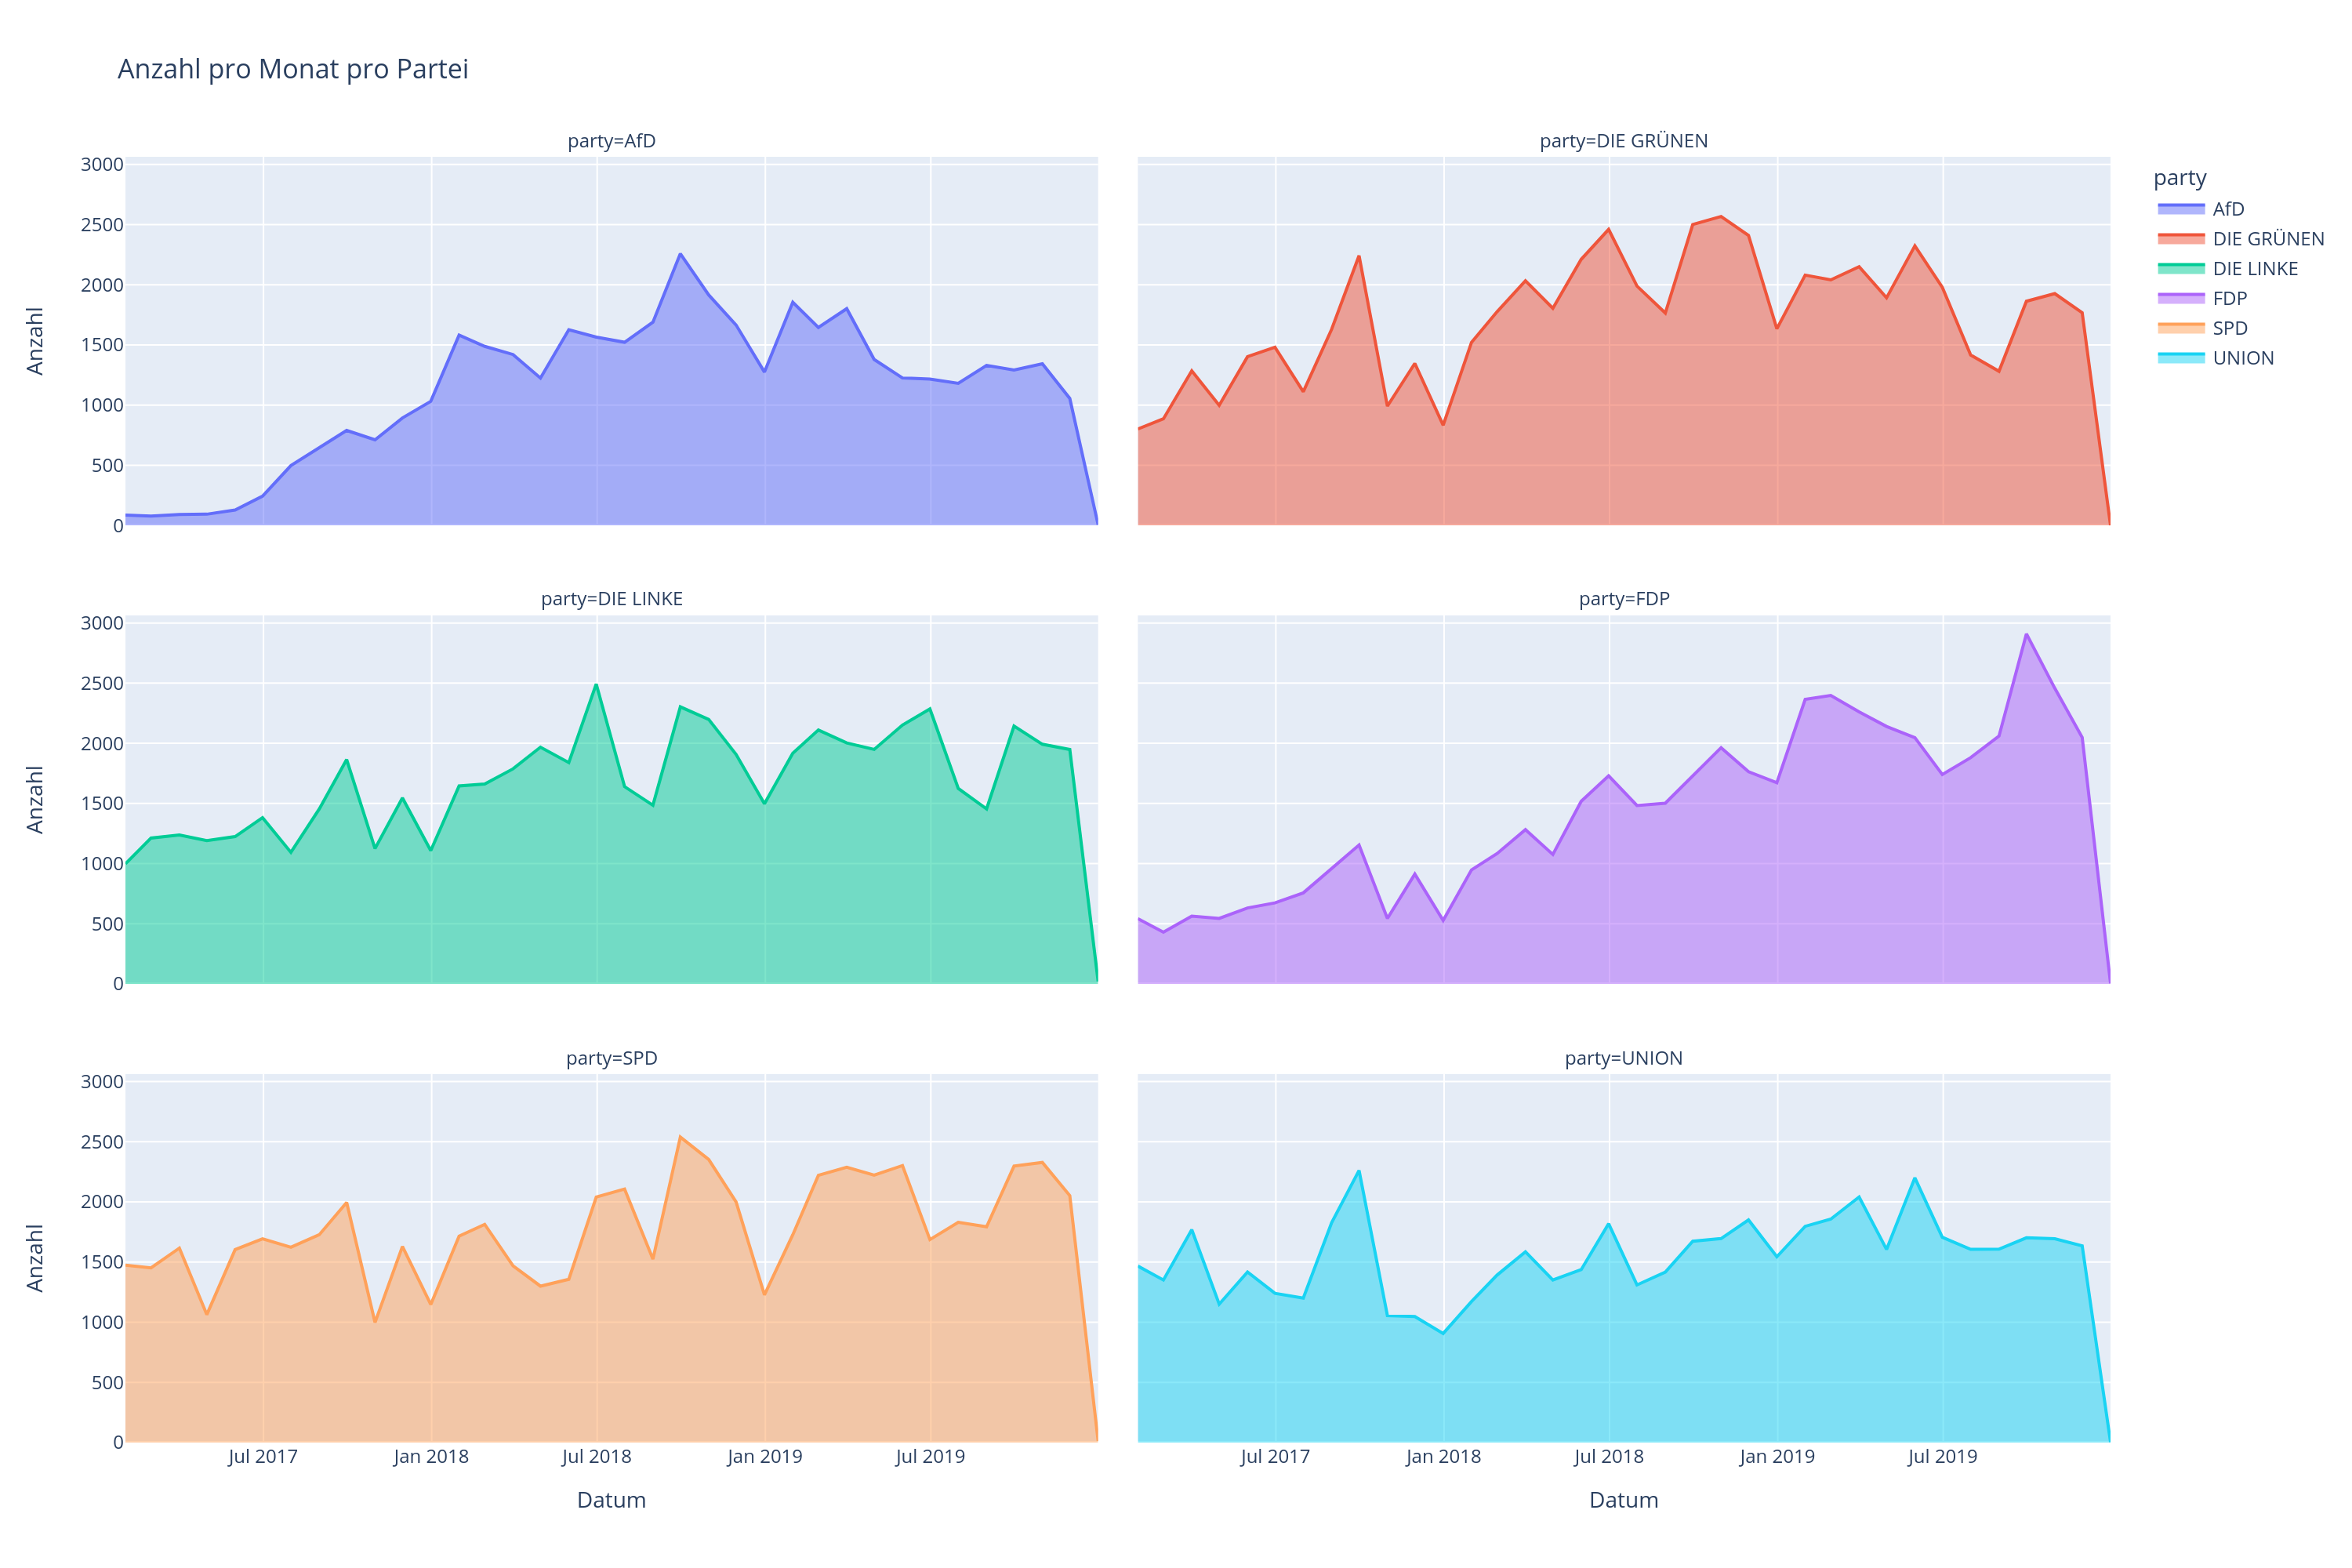
\includegraphics[width=\linewidth]{data/images/anzahl_pro_monat_pro_partei.png}
    \caption{Anzahl an Tweets pro Monat nach Partei} \label{fig:countTweetsTimeline}
\end{figure}

% TODO: Check wether to round 2 or 4

\begin{table}[H]
    \centering
    {\footnotesize
    \begin{tblr}{width=\textwidth, hlines, vlines} 
        \textbf{Partei} & \textbf{Negative} & \textbf{Neutral} & \textbf{Positive} \\
        
        AfD & \num{0.28} & \num{0.68} & \num{0.04} \\
        DIE GRÜNEN & \num{0.20} & \num{0.74} & \num{0.06} \\
        DIE LINKE & \num{0.21} & \num{0.75} & \num{0.04} \\
        FDP & \num{0.22} & \num{0.73} & \num{0.05} \\
        SPD & \num{0.18} & \num{0.74} & \num{0.09} \\
        UNION & \num{0.16} & \num{0.78} & \num{0.07} \\
    \end{tblr}
    }
    \caption{Prozentuale Sentimentverteilung} \label{tab:sentimentDistributionTweet}
\end{table}

\begin{figure}[H]
    \centering
    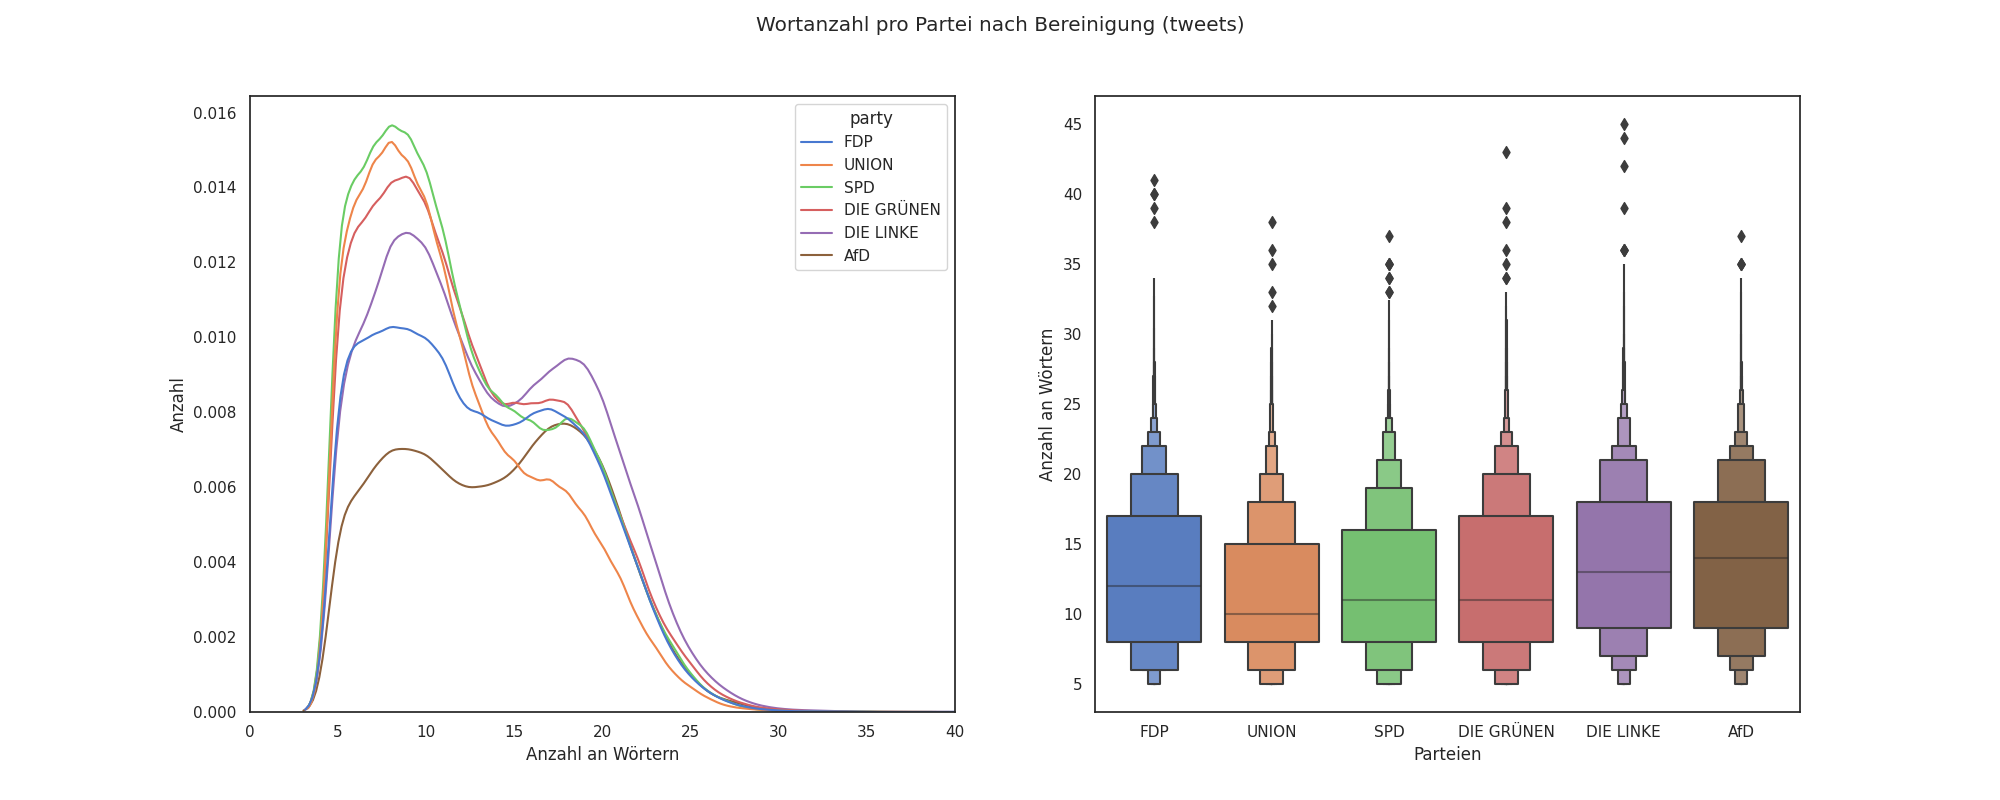
\includegraphics[width=\linewidth]{data/images/wortanzahl_pro_partei_nach_bereinigung.png}
    \caption{Wortanzahl pro Partei nach Bereinigung} \label{fig:countPartyCleaned}
\end{figure}

\section{Modeling} \label{sec:modeling}

% TODO: Review and add ideas for modeling

\begin{itemize}
    \item Datenquellen erst einzeln trainieren
    \item Datenquellen in verschiedenen Kombinationen trainieren
    \item Undersampling nach Partei 
\end{itemize}

\subsection{Feature Engineering} \label{subsec:featureEngineering}

% TODO: This are only ideas and options for additional features 
% TODO: Evaluate the features

\subsubsection{Sentiment}

Eine Limitation von den herkömmlichen \ac{ML} Modellen ist die Klassifikation von Polysemie \autocite[48\psq]{kowsari_text_2019}. 

% TODO: Find source

Ein Ansatz, um diese Limitation zu mindern, ist es, den Sentiment eines Textes zu berechnen. Ziel dieser Technik ist es nicht nur festzustellen, ob sich ein Politiker zum Beispiel zur \ac{AfD} äußert oder nicht, sondern ebenfalls, ob seine Äußerungen positiv, neutral oder negativ sind.

% TODO: Add timeline for ML Models

Die einfachste Methode, um den Sentiment von deutschen Texten zu ermitteln, sind Sentiment-Wörterbücher wie \textit{SentiWS}, \textit{BAWL-R} und \textit{GermanPolarityClues} \autocite[1627\psq]{guhr_training_2020}. CNN, SVM, Bi-LSTM, \dots

Die bisherigen regelbasierten Ansätze, als auch \ac{ML} Modelle wie \acp{SVM}, \acp{CNN} und \acp{LSTM} erreichen einen F1-Score von bis zu \num{74.9}. Alternativ zu diesen Ansätzen stellen \textcite{guhr_training_2020} ein \ac{BERT}-basiertes \ac{ML} Modell bereit. Dieses wurde mittels der folgenden Datensätze trainiert: \textit{PotTS}, \textit{SB10k}, \textit{GermEval-2017}, \textit{Scare}, \textit{Filmstarts}, \textit{holidaycheck}, \textit{leipzig-wikipedia} und \textit{Emotions}. Das Modell erreicht einen F1-Score von \num{0.9636} und ist somit den vorherigen Modellen deutlich überlegen \autocite[1631]{guhr_training_2020}.

\subsubsection{Gendern}

- Verhältnis Wörter/Gendersterne oder True/False
- Check mit RegEx ob gegendert wird und setze variable

\subsubsection{Dokumenttyp}

- Tweet, Speech, \dots

\subsection{Baseline Models}

% TODO: Update scores

\begin{table}[H]
    \centering
    {\footnotesize
    \begin{tblr}{width=\textwidth, hlines, vlines}
        \textbf{Modell} & \textbf{Datensatz} & \textbf{Precision} & \textbf{Recall} & \textbf{\(F_1\) Score} \\ 

        \textbf{SVM + \acs{BoW}} & Tweets & \num{0.59} & \num{0.59} & \num{0.59} \\
        \textbf{SVM + \acs{BoW}} & Wahlpro\-gramme & \num{0} & \num{0} & \num{0} \\
        \textbf{SVM + \acs{BoW}} & Reden & \num{0} & \num{0} & \num{0} \\

        \textbf{Kombiniert} & \textbf{\num{0}} & \textbf{\num{0}} & \textbf{\num{0}} \\
    \end{tblr}
    }
    \caption{Scores für Baseline Modelle auf Basis von \ac{BoW} und \ac{TF-IDF}} \label{tab:overviewScoresBaseline}
\end{table}

\subsection{Advanced Models}

\subsubsection{FastText}

% TODO: Update and add plots for other datasets

\begin{figure}[H]
    \begin{subfigure}{.5\textwidth}
      \centering
      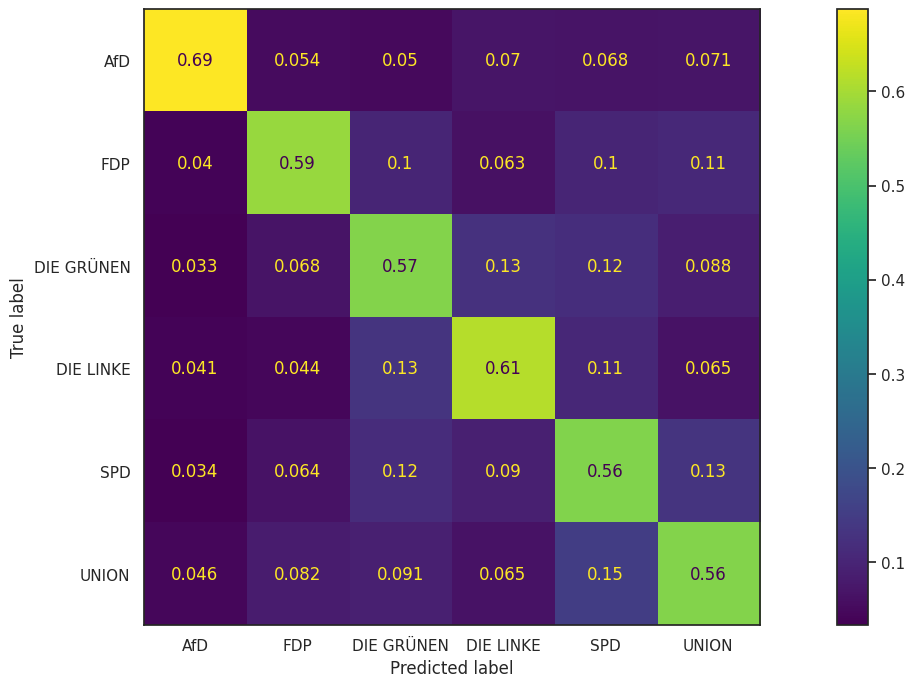
\includegraphics[width=0.9\linewidth]{data/images/fasttext_tweets_confusion.png}
      \caption{Tweets von \acs{MdB}} \label{sfig:confusionMatrixFastTextTweets}
    \end{subfigure}
    \begin{subfigure}{.5\textwidth}
      \centering
      \missingfigure{Wahlprogramme}
      \caption{Wahlprogramme} \label{sfig:confusionMatrixFastTextManifest}
    \end{subfigure}
    \begin{subfigure}{.5\textwidth}
      \centering
      \missingfigure{Reden}
      \caption{Reden im Deutschen Bundestag} \label{sfig:confusionMatrixFastTextSpeeches}
    \end{subfigure}
    \begin{subfigure}{.5\textwidth}
      \centering
      \missingfigure{Kombiniert}
      \caption{Kombinierten Datensatz} \label{sfig:confusionMatrixFastTextAll}
    \end{subfigure}
    \caption{Konfusion Matritzen für \texttt{fasttext}} \label{fig:confusionMatrixFastText}
\end{figure}

\begin{itemize}
    \item Parteien, welche politisch näher beieinander liegen, lassen sich schlechter Klassifizieren
\end{itemize}

% TODO: Update scores

\begin{table}[H]
    \centering
    {\footnotesize
    \begin{tblr}{width=\textwidth, hlines, vlines}
        \textbf{Datensatz} & \textbf{Precision} & \textbf{Recall} & \textbf{\(F_1\) Score} \\ 

        Tweets & \num{0.59} & \num{0.59} & \num{0.59} \\
        Wahlpro\-gramme & \num{0} & \num{0} & \num{0} \\
        Reden & \num{0} & \num{0} & \num{0} \\

        \textbf{Kombiniert} & \textbf{\num{0}} & \textbf{\num{0}} & \textbf{\num{0}} \\
    \end{tblr}
    }
    \caption{Scores für Supervised Learning mittels \texttt{fasttext} (\texttt{weighted avg})} \label{tab:overviewScoresFastText}
\end{table}

\subsubsection{BERT}

Lorem Ipsum

\subsubsection{ELMo}

Lorem Ipsum

\subsection{Limitationen}

\subsubsection{Feature Engineering}

% TODO: Add example for polysemy

Durch Methoden wie \ac{BoW} und \ac{TF-IDF} gehen syntaktische, als auch semantische Zusammenhänge verloren \autocite[48\psq]{kowsari_text_2019}. Dies führt dazu, dass Modelle wie \ac{SVM} und Random Forest ausschließlich die verwendeten Wörter und deren Anzahl in Betracht zieht, aber nicht die tiefere Bedeutung im Kontext des Satzes. Nach \textcite{kowsari_text_2019} versuchen Modelle wie Word2Vec, GloVe und \texttt{fasttext} zumindest syntaktische und semantische Zusammenhänge zu berücksichtigen, jedoch haben selbst diese Modelle Schwierigkeiten, Polysemie\footnote{Sätze mit mehreren Bedeutungen} zu klassifizieren.

\subsubsection{Sprache}

% TODO: Add sources and examples

Des Weiteren ergibt sich aus der Wahl der Datenquellen (Wahlprogramme, Reden und Tweets) eine Annahme/Voraussetzung/Bias geben über der verwendeten Sprache. Wahlprogramme, Reden und Tweets von Politikern weisen zwar parteispezifische Wörter auf, jedoch ist die semantische und syntaktische Komplexität der Sätze überdurchschnittlich hoch. Ebenfalls ist die Menge an Rechtschreibfehlern und verwendetem Slang geringer als bei anderen Textarten. Daraus folgt, dass die Performance der trainierten Modelle voraussichtlich signifikant schlechter ist, wenn Texte sprachlich (semantisch und syntaktisch) stark von den Trainingsdaten abweichen.

\subsubsection{Politische Nähe}

% TODO: Add sources and image
% TODO: Reason --> Politisches Viereck (links -- rechts, ...)

Parteien, welche ähnliche politische Ideale verfolgen, identische Themenschwerpunkte haben, lassen sich schlechter klassifizieren.

\section{Fazit} \label{sec:crispConclusion}

\begin{itemize}
    \item Gendern nicht kompatibel mit Lemmatizing und daher problematisch
\end{itemize}
